% ============================================================================
% 2026-09-29: the shift (dating) test re-run for the HEADLINE forecast under the
% 16:00-bar recalibration of Table~\ref{tab:close_option_rules}.  Every number
% below is a macro from generated/appendix_close_shift_test.tex, written by
% experiments/close_shift_test_headline.py from
% results/close_shift_test/shift_test_headline.csv; nothing is typed by hand.
% The notebook's own shift test (Section~\ref{sec:app_run_parked}, the paper's
% eight forecasts under the session-bar recalibration) is a different scorer and
% is not set beside this one.  Input from main.tex after
% sections/appendix_running_parked, so this continues Appendix D.
% ============================================================================
% AUTO-GENERATED by experiments/close_shift_test_headline.py from results/close_shift_test/shift_test_headline.csv -- do not edit.
\begingroup\scriptsize\setlength{\tabcolsep}{1pt}
\begin{longtable}{llrrrrll}
\caption{The shift (dating) test of the headline forecast under the 16:00-bar recalibration: the 15:30 $\mathrm{sign}(s)$ rule with the forecast row shifted by $k$ half-hour bars, every row placed on the traded bar's scale, on the 865 deck days for which every shifted row exists. $k<0$: the same session's earlier row; $k=0$: the trade; $k>0$: the next session's row (the headline has session rows only), whose lags contain the traded bar. $\Delta$ is against $k=0$ with the paired day-block 95\,\% interval.}\label{tab:app_shift_test_headline}\\
\toprule
row & row read & Sharpe mid & Sharpe crossed & buy \% & agree \% & $\Delta$ mid [95\,\%] & $\Delta$ crossed [95\,\%] \\
\midrule
\endfirsthead
\caption[]{(continued)}\\
\toprule
row & row read & Sharpe mid & Sharpe crossed & buy \% & agree \% & $\Delta$ mid [95\,\%] & $\Delta$ crossed [95\,\%] \\
\midrule
\endhead
\bottomrule
\endlastfoot
$k=$-12 & 10:00, same & 0.12 & -0.35 & 49 & 69 & -1.73 [-2.91, -0.57] & -1.74 [-2.92, -0.57] \\
$k=$-11 & 10:30, same & -0.31 & -0.78 & 48 & 69 & -2.17 [-3.34, -1.03] & -2.17 [-3.35, -1.02] \\
$k=$-10 & 11:00, same & -0.03 & -0.50 & 48 & 66 & -1.88 [-3.07, -0.67] & -1.89 [-3.08, -0.67] \\
$k=$-9 & 11:30, same & 0.35 & -0.13 & 43 & 68 & -1.50 [-2.70, -0.28] & -1.51 [-2.71, -0.28] \\
$k=$-8 & 12:00, same & 0.42 & -0.05 & 46 & 70 & -1.44 [-2.52, -0.36] & -1.44 [-2.53, -0.36] \\
$k=$-7 & 12:30, same & 0.51 & 0.03 & 42 & 69 & -1.35 [-2.47, -0.22] & -1.36 [-2.49, -0.23] \\
$k=$-6 & 13:00, same & 0.64 & 0.17 & 44 & 69 & -1.21 [-2.46, +0.07] & -1.22 [-2.48, +0.07] \\
$k=$-5 & 13:30, same & 0.95 & 0.47 & 38 & 70 & -0.91 [-1.92, +0.11] & -0.91 [-1.93, +0.11] \\
$k=$-4 & 14:00, same & 0.93 & 0.45 & 37 & 71 & -0.93 [-2.11, +0.21] & -0.94 [-2.11, +0.21] \\
$k=$-3 & 14:30, same & 1.29 & 0.80 & 26 & 72 & -0.57 [-1.67, +0.46] & -0.59 [-1.69, +0.45] \\
$k=$-2 & 15:00, same & 0.50 & 0.02 & 25 & 71 & -1.35 [-2.72, -0.01] & -1.37 [-2.74, -0.02] \\
$k=$-1 & 15:30, same & -0.00 & -0.47 & 32 & 75 & -1.86 [-2.96, -0.78] & -1.86 [-2.96, -0.79] \\
$k=$+0 & 16:00, same & 1.85 & 1.39 & 40 & 100 & +0.00 [+0.00, +0.00] & +0.00 [+0.00, +0.00] \\
$k=$+1 & 10:00, next & 0.88 & 0.41 & 44 & 68 & -0.97 [-2.22, +0.31] & -0.97 [-2.24, +0.32] \\
$k=$+2 & 10:30, next & 0.93 & 0.46 & 44 & 68 & -0.92 [-1.91, +0.12] & -0.92 [-1.91, +0.13] \\
$k=$+3 & 11:00, next & 1.00 & 0.53 & 41 & 66 & -0.85 [-2.12, +0.45] & -0.86 [-2.12, +0.46] \\
$k=$+4 & 11:30, next & 0.83 & 0.36 & 42 & 66 & -1.02 [-2.30, +0.26] & -1.03 [-2.31, +0.26] \\
$k=$+5 & 12:00, next & 1.22 & 0.75 & 41 & 65 & -0.63 [-1.93, +0.63] & -0.64 [-1.95, +0.63] \\
$k=$+6 & 12:30, next & 1.51 & 1.04 & 42 & 63 & -0.34 [-1.66, +0.89] & -0.35 [-1.67, +0.90] \\
realized (target) & 16:00 (traded bar) & 4.48 & 4.02 & 27 & 67 & +2.63 [+1.21, +4.17] & +2.63 [+1.20, +4.17] \\
realized (unclipped) & 16:00 (traded bar) & 4.50 & 4.03 & 27 & 67 & +2.64 [+1.22, +4.19] & +2.65 [+1.21, +4.19] \\
always short &  & 0.27 & -0.22 & 0 & 60 & -1.58 [-2.98, -0.13] & -1.60 [-3.00, -0.16] \\
\end{longtable}
\endgroup

\newcommand{\shiftNDays}{865}
\newcommand{\shiftBarZeroMid}{1.85}
\newcommand{\shiftBarZeroCrossed}{1.39}
\newcommand{\shiftBarZeroAllMid}{1.90}
\newcommand{\shiftBarZeroAllCrossed}{1.44}
\newcommand{\shiftMinusOneMid}{-0.00}
\newcommand{\shiftMinusOneDelta}{-1.86}
\newcommand{\shiftMinusOneLo}{-2.96}
\newcommand{\shiftMinusOneHi}{-0.78}
\newcommand{\shiftBestStaleRow}{-3}
\newcommand{\shiftBestStaleMid}{1.29}
\newcommand{\shiftBestStaleDelta}{-0.57}
\newcommand{\shiftBestStaleLo}{-1.67}
\newcommand{\shiftBestStaleHi}{+0.46}
\newcommand{\shiftNStaleAbove}{0}
\newcommand{\shiftNStaleIntervalAbove}{0}
\newcommand{\shiftNStaleIntervalBelow}{8}
\newcommand{\shiftPlusOneMid}{0.88}
\newcommand{\shiftPlusOneCrossed}{0.41}
\newcommand{\shiftPlusOneDelta}{-0.97}
\newcommand{\shiftPlusOneLo}{-2.22}
\newcommand{\shiftPlusOneHi}{+0.31}
\newcommand{\shiftNextMinMid}{0.83}
\newcommand{\shiftNextMaxMid}{1.51}
\newcommand{\shiftNNextIntervalAbove}{0}
\newcommand{\shiftStarMid}{4.48}
\newcommand{\shiftStarCrossed}{4.02}
\newcommand{\shiftAlwaysShortMid}{0.27}
\newcommand{\shiftMinusOneAgree}{75}
\newcommand{\shiftPlusOneAgree}{68}

\subsection{The Shift (Dating) Test of the Headline Forecast}
\label{sec:app_shift_test_headline}

\paragraph{What is tested.} The last-30-min trade reads the per-bar ridge's row
labelled 16:00 --- the forecast of the 15:30--16:00 bar, issued at 15:30. The test
re-scores the $\mathrm{sign}(s)$ rule with the forecast \emph{row} shifted by $k$
half-hour bars and everything else unchanged. For $k<0$ the rule reads the same
session's earlier row (the 15:30 row at $k=-1$, down to the 10:00 row at $k=-12$): a
stale forecast, still free of look-ahead. For $k>0$ the headline, a per-bar model with
session rows only, has no row after the close; the rule reads the \emph{next}
session's row (10:00 at $k=+1$, to 12:30 at $k=+6$), the first rows whose lag ladder
contains the traded bar. Because another row forecasts another bar, every shifted row
is placed on the traded bar's own scale, $(\hat y_k^2+\hat s_{16{:}00})\,B_{16{:}00}$,
with the smear $\hat s$ and profile $B$ the trade itself uses, so the only thing that
changes with $k$ is what the model had seen; at $k=0$ this is the trade's forecast
(gated). The star is the traded bar's realized variance in place of the forecast.
Scorer, trade, fills and intervals are those of Table~\ref{tab:close_option_rules};
the \shiftNDays{} deck days for which every shifted row exists are scored (the last
deck day has no next session, and two sessions lack the 10:00--11:00 rows), and at
$k=0$ on all 866 days the rule reproduces Table~\ref{tab:close_option_rules}
(\shiftBarZeroAllMid{} mid, \shiftBarZeroAllCrossed{} crossed).

\paragraph{Reading.} Table~\ref{tab:app_shift_test_headline} gives every row.
One bar stale, the rule falls from \shiftBarZeroMid{} to \shiftMinusOneMid{}
($\Delta$ \shiftMinusOneDelta{} [\shiftMinusOneLo{}, \shiftMinusOneHi{}]); its
position agrees with the trade's on \shiftMinusOneAgree{}\,\% of days. Of the twelve
stale rows, \shiftNStaleAbove{} sit above $k=0$ in point estimate,
\shiftNStaleIntervalBelow{} have an interval below zero and
\shiftNStaleIntervalAbove{} an interval above; the best stale row is
$k=\shiftBestStaleRow$ at \shiftBestStaleMid{} ($\Delta$ \shiftBestStaleDelta{}
[\shiftBestStaleLo{}, \shiftBestStaleHi{}]). The next session's rows, placed on the
traded bar's scale, score \shiftNextMinMid{} to \shiftNextMaxMid{} at the midpoint
(\shiftNNextIntervalAbove{} of six intervals above zero; $k=+1$: \shiftPlusOneMid{}
mid, \shiftPlusOneCrossed{} crossed, $\Delta$ \shiftPlusOneDelta{}
[\shiftPlusOneLo{}, \shiftPlusOneHi{}], agreement \shiftPlusOneAgree{}\,\%), and
the realized variance itself scores \shiftStarMid{} mid, \shiftStarCrossed{}
crossed, against always short at \shiftAlwaysShortMid{} on the same days. The
next-session rows are a different probe from the notebook's after-hours rows
(Section~\ref{sec:app_run_parked}): each is a separate regression for its own bar,
so the traded bar enters through that regression's own lag weights rather than
through the traded row's, and the two tests are not compared.

\begin{figure}[H]
\centering
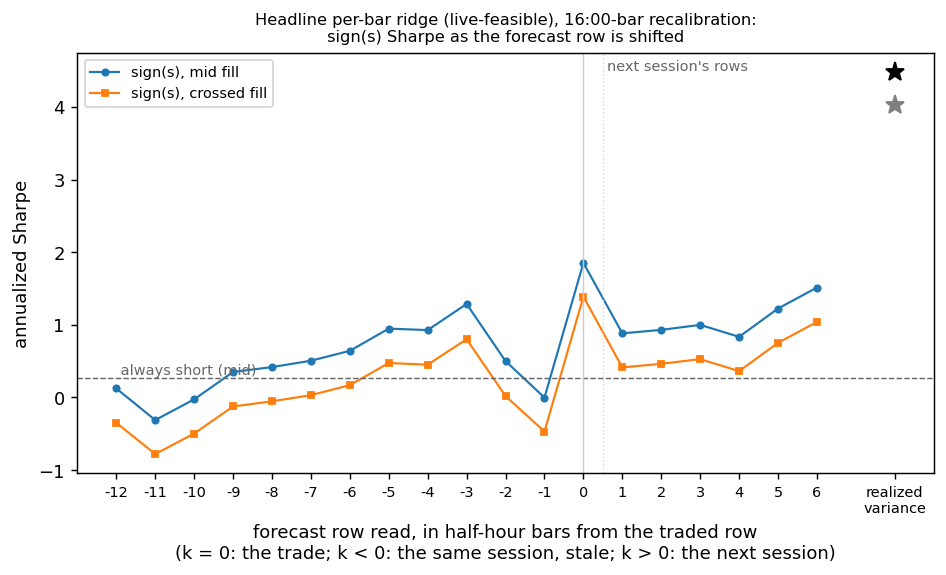
\includegraphics[width=\textwidth]{../results/close_shift_test/shift_test_headline.png}
\caption{The headline forecast's $\mathrm{sign}(s)$ Sharpe as the forecast row is
shifted, on the same \shiftNDays{} days (source:
\texttt{results/close\_shift\_test/shift\_test\_headline.csv}).}
\label{fig:app_shift_test_headline}
\end{figure}
